\documentclass[12pt,fleqn]{article}\usepackage{../../common}
\begin{document}
Gazlar, Sıvılar - 2

Taşınımsal Nakil (Convective Transport)

Bu kavramı anlamak için bir akışın önünde duran geçirgen bir yüzey
düşünelim. Akışı temsil eden hız alanını biliyoruz, bu alanın yüzeydeki
vektörleri bir sıvı parçacığının o noktadaki, o andaki hareketini gösteriyor.

Bir sıvı parçacığı yeri değiştirilebilecek belli oranda bir madde, öğe
içerebilir, ve o parçacık yüzeyin bir tarafından diğer tarafına geçtiğinde
parçacıkla beraber ögenin yeri de değişmiş olur. Dikkat nakletme direk bir
geçiş ima eder, hızın normal bileşenine oranla bir geçiştir bu. Bu bağlamda
hızın sadece normal (yüzeye dik) olan bileşenine bakarız, çünkü yüzeye
teğet olan bileşen hiç bir geçiş oluşturmazdı, yüzeye paralel olan bir
gidiştir bu. Tabii ki yüzeyin farklı noktalarında farklı hızlar, ve farklı
öğe değerleri olabilir, bu sebeple taşınımsal naklinin matematiksel
tarifi bu farklılıkları göz önüne almalıdır. 

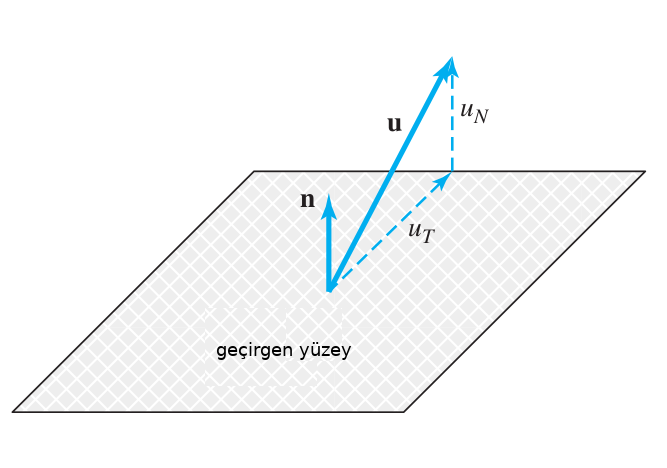
\includegraphics[width=20em]{phy_030_fluid2_04.png}

Şimdi taşınımsal nakil $\Gamma_C$ ile tanımlarsak, bu değişken bir zaman anında
sıvının akışı sebebiyle bir öğenin yüzeyi geçme oranı olacaktır. Eğer $\epsilon$
birim kütledeki öğe miktarı ise, $\rho \epsilon$ birim hacimdeki o öğenin
miktarı olur (çünkü $\rho$ yoğunluk, birim hacimdeki kütle). O zaman herhangi
bir noktada bu ögenin hız alanı içinde yerel bir hız vektörü yönünde anlık
taşınma oranı / hızı $\rho \epsilon u$ olur, $u = \bar{u}(\bar{x},t)$. Bu
oranı yüzeyden geçise tercüme edersek, yüzeydeki $n$ normaline sahip $\ud S$
yüzey alanından geçiş oranı

$$
\delta \Gamma_C = \rho \epsilon (u \cdot n) \ud S
$$

Daha önce belirttik yüzeyin her noktasında farklı nakil oranları olabilir,
tüm geçirgen yüzey için $\Gamma_C$ hesabı için her yüzey ögesinden olan geçiş
oranlarını bir yüzey entegrali ile toplarız,

$$
\Gamma_C = \int_S \rho \epsilon (u \cdot n) \ud S
$$

Bu tür entegrallere taşınımsal akış entegrali (convective flux integral) ya da
kısaca taşınımsal entegral ismi veriliyor. Fakat dikkat bu hesabın sonucu bir
oran (birim zamandaki öğe), akış değil (birim alandaki öğenin birim zamandaki
hızı).

Kabaca öğe dedik, ama pek çok kavram üstteki formüller kapsamına giriyor, mesela
kütle hesabı için $\epsilon = 1$ diyebiliriz, ya da momentum için
$\epsilon = u$. Isı taşınımı da benzer şekilde temsil edilir.

Reynolds Nakletme Teorisi (Reynold's Transport Theorem)

Daha önce pür kütle hesabında $\epsilon = 1$ üzerinden türetilen muhafaza
kanununu görmüştük,

$$
\frac{\partial \rho}{\partial t} + \nabla \cdot (\rho u ) = 0
$$

Ya da 

$$
\frac{\partial \rho}{\partial t} + \bdiv (\rho u ) = 0
\mlabel{1}
$$

Bu $\epsilon = 1$ durumudur, daha genel $\epsilon$ için

$$
\frac{\partial \rho \epsilon}{\partial t} + \bdiv (\rho \epsilon u ) = 0
$$

elde edileceğini ispat etmek zor değil. Terim $\bdiv$ içindekilere çarpım
kuralını uygularsak, ve $\epsilon$ yerine $\phi$ kullanınca açılım [3, sf. 24]

$$
\rho \frac{\partial \phi}{\partial t} +
\phi \frac{\partial \rho}{\partial t} + 
\rho \bdiv (\phi u ) +
\phi \bdiv (\rho u ) = 0
$$

$$
\rho \frac{\partial \phi}{\partial t} +
\phi \bdiv (\rho u ) +
\phi \left(
  \frac{\partial \phi}{\partial t} + \bdiv (\rho u ) 
\right) = 0
$$

Akış alanı süreklilik kuralını destekliyor, yani (1) geçerli, o zaman
parantez içindekiler yok sayılır,

$$
\rho \frac{\partial \phi}{\partial t} + \phi \bdiv (\rho u ) = 0
$$

Üstteki formülü kontrol hacmi $V$ üzerinden entegre edip Gauss'un uzaklaşım
teorisini uygulayınca,

$$
\iiint_V \left(
\rho \frac{\partial \phi}{\partial t} + \phi \bdiv (\rho u )
\right) \ud V =
\iiint_V \rho \frac{\partial \phi}{\partial t} +
\oint \oint_S \phi u \cdot n \ud S
\mlabel{2}
$$

Reynolds nakletme teorisi budur. Eşitliğin sağ tarafının sıfıra eşit olduğunu
düşününce ifadenin söylediği $\phi$'deki değişim oranının kontrol hacmi
üzerindeki akışların (flux) net dengesine eşit olduğudur; denge derken girenler
eksi çıkan akışların net toplamı [3, sf. 25].

Momentum Dengesi

Kütle aktarıldığı gibi momentum da aktarılabilir, ve bir kontrol hacminde
incelenebilir. Önce Newton'un kanununu hatırlayalım,

$$
\frac{\ud (m u)}{\ud t} = F
$$

ki $F$ ve $u$ vektör. Momentumun muhafaza edildiğini vurgulamak için Newton'un
kanununu sabit kontrol hacmi üzerinden entegre edelim, ve sağ tarafta bu
Reynolds nakil teorisinin momentum muhafaza formuna tekabül edecektir. O sağ
taraf nasıl formülize edilir? Daha önce $\epsilon = 1$ ile kütle $\epsilon = u$
ile momentum formülüne erisebileceğimizi söylemiştik. Ya da Reynolds nakil
formülü (2)'de $\phi = \rho u$ ile momentum dengesi elde edebiliriz [3, sf. 26],

$$
\iiint_V \frac{\ud (m u)}{\ud t} \ud V =
\iiint_V \rho \frac{\partial u}{\partial t} \ud V +
\oint \oint_S \rho u u \cdot n \ud S =
\iiint_V F \ud V
\mlabel{3}
$$

Muhafaza Kanunları Tek Boyut

İçinde gaz olan sadece tek boyutuna baktığımız bir tüp düşünelim, $x$ tüpün
üzerindeki bir noktayı temsil edecek, $\rho(x,t)$ ise tüpün $x$ noktasında ve
$t$ anındaki yoğunluğunu verecek diyelim. Yoğunluğu kullanarak $x_1$ ve $x_2$
noktaları arasındaki $t$ anındaki kütle

$$
\int _{x_1}^{x_2} \rho(x,t) \ud x
$$

ile hesaplanabilir. Tüpün duvarları tam izole ise ve kütle yoktan varedilip
yokedilemeyeceğine göre tüpe gaz giriş ya da çıkış sadece $x_1,x_2$
noktalarından olabilir [4, sf. 14]. Şimdi bir gaz hareket hızı düşünelim,
$u(x,t)$ ile, o zaman gaz akma oranı, ya da akış (flux)

$$
flux = \rho(x,t) u(x,t)
$$

olur. Üstteki fiziksel kurallardan hareketle $[x_1,x_2]$ deki kütlenin
değişim oranı $x_1$ ve $x_2$ noktalarındaki akışın farkına eşit olmalıdır,

$$
\frac{\ud}{\ud t} \int _{x_1}^{x_2} \rho(x,t) \ud x =
\rho(x_1,t) u(x_1,t) - \rho(x_2,t) u(x_2,t)
$$

İşte bu muhafaza kanununun entegral formudur. 

Üstteki formülü $t_1,t_2$ zaman aralığı için entegre edersek, ki böylece
bu zaman içindeki tüm toplam akışı hesaplayabilelim, o zaman

$$
\int_{t_1}^{t_2} \left( \frac{\ud}{\ud t} \int _{x_1}^{x_2} \rho(x,t) \ud x  \right)  =
\int_{t_1}^{t_2} \rho(x_1,t) u(x_1,t) \ud t -
\int_{t_1}^{t_2} \rho(x_2,t) u(x_2,t) \ud t
$$

Soldaki kısım zaman üzerinden türevin yine zaman üzerinden entegrali, o zaman
yokolabilir, Calculus'un Temel Teorisi üzerinden basitleştirirsek,

$$
\int _{x_1}^{x_2} \rho(x,t_2) \ud x -
\int _{x_1}^{x_2} \rho(x,t_1) \ud x  = 
\int_{t_1}^{t_2} \rho(x_1,t) u(x_1,t) \ud t -
\int_{t_1}^{t_2}  \rho(x_2,t) u(x_2,t) \ud t
$$

Ufak bir yer değiştirme sonrası

$$
\int _{x_1}^{x_2} \rho(x,t_2) \ud x =
\int _{x_1}^{x_2} \rho(x,t_1) \ud x  +
\int_{t_1}^{t_2} \rho(x_1,t) u(x_1,t) \ud t -
\int_{t_1}^{t_2}  \rho(x_2,t) u(x_2,t) \ud t
$$

Üstteki formun değişik bir şekli ileride lazım olacak, zaman adımı atmaya
uğraştığımız hesapsal yöntemlerde $t_1$ ve $t_2$ üzerinden bir entegral, hesabı
bir sonraki zamana geçirmeye uğraştığımızda, adım attığımızda.

Neyse şimdi diferansiyel forma geçise dönelim. Bu noktada $\rho(x,t)$ ve
$u(x,t)$'nin türevi alınabilir fonksiyonlar olduğunu farz ediyoruz. Üstekini,
yine ufak bir değişim sonrası,

$$
\int _{x_1}^{x_2} \rho(x,t_1) \ud x  +
\int _{x_1}^{x_2} \rho(x,t_2) \ud x -
\int_{t_1}^{t_2}  \rho(x_2,t) u(x_2,t) \ud t -
\int_{t_1}^{t_2} \rho(x_1,t) u(x_1,t) \ud t = 0
\mlabel{4}
$$

olarak görelim. Eğer Calculus'un Temel Teorisi ile ilk iki terime
$\int_{t_1}^{t_2} .. \ud / \ud t$ son iki terime $\int_{x_1}^{x_2} .. \ud / \ud x$
ekleyebilirsek, tüm terimlerde aynı entegraller olacağı için, 
$\int_{t_1}^{t_2} \int_{x_1}^{x_2} $ altında tüm terimleri gruplayıp
basitleştirmek mümkün, ve bunlar sıfıra eşit olur. Bu bizi diferansiyel
forma götürebilir. Yani

$$
\rho(x,t_2) - \rho(x,t_1) = \int_{t_1}^{t_2}
\frac{\partial }{\partial t} \rho(x,t) \ud t
$$

ve

$$
\rho(x_2,t)u(x_2,t) - \rho(x_1,t)u(x_1,t) =
\int _{x_1}^{x_2} \frac{\partial }{\partial x} (\rho(x,t)u(x,t)) \ud x
$$

eşitliklerinden hareketle, bunları (4)'e uygulayıp

$$
\int _{t_1}^{t_2} \int _{x_1}^{x_2}  \left\{
\frac{\partial }{\partial t} \rho(x,t)  +
\frac{\partial }{\partial x} (\rho(x,t)u(x,t))
\right\} \ud x \ud t = 0
\mlabel{4}
$$

elde ediyoruz. Bu ifadenin $[x_1,x_2]$ ve $[t_1,t_2]$ arasındaki tüm değerlerde
doğru olması gerektiği için entegre edilenin sıfır olması gerekiyor ([5]'dekine
benzer bir mantık yürütüldü), yani

$$
\rho_t + (\rho v)_x = 0
$$

olmalı. Böylece kütlenin muhafaza kuralını diferansiyel formda elde etmiş olduk.

Bu formu izole halde çözmenin tek yolu $v$'nin önceden bilindiği durumdadır, ya
da $v$ fonksiyon $\rho(x,t)$'ye bağlı bir fonksiyon olmalıdır, yani
$f(\rho) = \rho v$ gibi. Bu durumda üstteki ifade $\rho$ için tek sayısal
muhafaza kanunu haline gelir,

$$
\rho_t + f(\rho)_x = 0
$$

Diğer Muhafaza Edilen Büyüklükler

Tekrar üzerinden geçip, genişletelim, [6, sf. 15] notasyonu ile devam edelim,
ölçmek istediğimiz sıkıştırılamayan bir sıvı, gaz büyüklüğü var, ve bunu $x$
noktasında $t$ anı için $q(x,t)$ ile ölçüyoruz, takip ediyoruz. Mesela sıvı
içine bir işaretleyici karıştırılmış, mürekkep gibi, o takip ediliyor. Takip
edilen bu ölçümün yoğunluğu $q(x,t)$ olsun, bu fonksiyonun ne olduğunu anlamak
istiyoruz. Bu işaretleyicinin $x_1$ ve $x_1$ arasındaki kütlesinin hesabı için

$$
\int _{x_1}^{x_2} q(x,t) \ud x
$$

hesaplanır. Şimdi akış (flux) kavramını tekrar tanıştıralım, herhangi bir $x$
noktasında ve $t$ anındaki işaretleyici yoğunluğunun akma oranı akistir.
Bilinen $u(x,t)$ hızı ve yoğunluk $q(x,t)$'yi çarparak onu elde edebiliriz,

$(x,t)$'deki akış  = $u(x,t) q(x,t)$

Dikkat, akış sıfırdan büyükse bu sağa doğru akış demektir, küçükse sola doğru
akış demektir. Hız bilinen bir büyüklük olduğuna göre bir akışı $f$'yi $q$'nun
fonksiyonu olarak yazabiliriz,

akış = $f(q,x,t) = u(x,t) q$ 

Şimdi üstteki entegral ile akış formülünü bağlayalım. Kütle muhafaza edildiği
için $x_1$ ve $x_2$ arasındaki kütleyi hesaplamıştık hatırlarsak, bu kütlenin
zamana göre değişim oranı sadece ve sadece o bölgeye sağdan ve solda olacak
akışlar ile mümkündür.

$$
\frac{\ud}{\ud t} \int _{x_1}^{x_2} q(x,t) \ud x =
f(q(x_1,t)) - f(q(x_2,t)) 
$$

Dikkat, $x_2$ üzerindeki akışta eksi işareti var çünkü sağdaki sınırdan
sola doğru akışı istiyoruz, ve $x_1$ üzerindeki akışta artı işaret var,
çünkü o sınırdan sağa doğru giden, $[x_1,x_2]$ bölgesine giren akışa
bakıyoruz.

Ustteki formulun sag tarafini Calculus'un standart notasyonu ile yazabiliriz,

$$
\frac{\ud}{\ud t} \int _{x_1}^{x_2} q(x,t) \ud x =
-f(q(x_1,t)) \biggr\rvert_{x_1}^{x_2}
$$

Calculus'a geçtiğimize göre sağ tarafı Calculus'un Temel Teorisi üzerinden
türevin entegrali haline çevirebiliriz,

$$
\frac{\ud}{\ud t} \int _{x_1}^{x_2} q(x,t) \ud x =
- \int_{x_1}^{x_2} \frac{\partial }{\partial x} f(q(x,t)) \ud x
$$

Şimdi zaman türevini entegral içine alabiliriz. Ayrıca eşitliğin sol ve sağ
kısmı aynı entegrale sahip oldukları için onları birleştirmek mümkün,

$$
\int _{x_1}^{x_2}
\left[
\frac{\ud}{\ud t} q(x,t) + \frac{\partial }{\partial x} f(q(x,t)) 
\right]
\ud x  = 0
$$

Daha önce (4) formülü için kullandığımız mantık geçerli, o zaman entegre
edilen sıfır olmalı, böylece alttaki diferansiyel denklemi elde ediyoruz,

$$
\frac{\ud}{\ud t} q(x,t) + \frac{\partial }{\partial x} f(q(x,t))  = 0
$$

Ya da

$$
q_t(x,t) + f(q(x,t))_x  = 0
$$

Aynen kütle muhafaza edildiği gibi momentum da muhafaza edilebilir. Bu durumda
$\rho(x,t) u(x,t)$ bir momentum yoğunluğu verir, ki $\rho$ kütle yoğunluğu, ve
$\rho u$ çarpımının iki nokta arasındaki entegrali o aralıktaki toplam momentumu
hesaplar, ve bu toplam sadece o aralığa sınırlardan girecek hareket eden sıvıyla
gelecek dış momentumlar ile değisebilir. Eğer $q = \rho u$ ise akış
$(\rho u) u = \rho u^2$ ile hesaplanır.

Fakat momentum hesabına etki eden başka faktörler de var. Üstteki makroskopik,
büyük ölçekteki bir etkiydi. Mikroskopik bir etki de var. Çünkü düşünürsek eğer
gaz hiç hareket etmiyor bile olsaydı, yani makroskopik görünen hız $u=0$
olsaydı, hala gaz içindeki moleküller hareket halinde olurdu [6, sf 292]. Öyle
değil mi?  Eğer gaz ısısı mutlak sıfır üzerinde ise bir hareket var
demektir. İşte bu hareketlilik gaz içinde basınç yaratır. Herhangi bir $x_1$
noktasındaki basıncı anlamak için tek boyutlu tüpümüzün o noktasına bir hayali
duvar soktuğumuzu düşünelim ve bu duvarın her iki tarafına gaz tarafından
uygulanacak kuvveti (birim alan bazlı olarak) hesaplayalım. Bu kuvvetler
normalde aynı mutlak büyüklükte ama ters işaretli olurlar. Fakat tüpün her
iki ucunu göz önüne alırsak eğer bu iki uçta basınç farkı var ise bu
iç titreşimlerin bir tarafta diğerine göre daha fazla olduğu anlamına gelir
ve bu fark bizim baktığımı tüp aralığına momentum eklenmesi olarak yansır.

O zaman momentum akışını $\rho u^2 + p$ olarak hesaplamak gerekir, entegral
muhafaza kanunu olarak,

$$
\frac{\ud}{\ud t} \int _{x_1}^{x_2} 
\rho(x,t) u(x,t) \ud x = - [\rho u^2 + p] _{x_1}^{x_2}
$$

Dikkat $[\hdots]_{x_1}^{x_2}$ işlemi ile iki uç arasındaki basınç farkını
formüle katmış oluyoruz.

Ve tekrar daha önce gördüğümüz matematiksel işlemleri yine uygularsak,
$\rho,u,p$'nin pürüzsüz fonksiyonlar olduğunu varsayarak momentum denkleminin
diferansiyel formunu elde edebiliriz,

$$
(\rho u)_t + (\rho u^2 + p)_x = 0
$$

Energy için de benzer bir taşınma formülü mümkün. $E$ sembolüyle birim hacimdeki
enerji yoğunluğunu temsil edelim, bu enerji de gaz akışı içinde taşınacaktır, bu
durum makroskopik akış terimi $E u$ sonucunu verir. Ayrıca mikroskopik seviyede
basınç $p$'nin yarattığı da kinetik enerjide bir $pu$ akışına sebep olacaktır.
Enerji denklemini o zaman,

$$
E_t + [(E + p) u ]_x = 0
$$

ile gösteririz. $E$ ile $p$'nin toplanmış olması garip gelebilir, birisi enerji
diğeri kuvvet. Fakat ölçüm birimlerini kontrol etmek gerekirse, $E$ ile birim
hacim, mesela $m^3$, içindeki enerji $N m$ var, basınç ise birim alandaki
kuvvettir, yani $N / m^2$. $E$ için $N m / m^3 = N / m^2$ elde edilir ki bu
basıncın birimi ile aynı.

Tum bu denklemleri biraraya koyunca, Euler Gaz Dinamigi formuller (Euler
Equation of Dynamics) elde edilir.

$$
\left[\begin{array}{c}
\rho \\ \rho u  \\ E
\end{array}\right]_t
+
\left[\begin{array}{c}
\rho u \\ \rho u^2 + p \\ (E+p) u 
\end{array}\right]_x 
= 0
$$


[devam edecek]

Kaynaklar

[1] Versteeg, {\em An Introduction to CFD}

[2] Katz, {\em Introduction to Fluid Mechanics}

[3] Mueller, {\em Essentials of Computational Fluid Mechanics}

[4] Leveque, {\em Numerical Methods for Conservation Laws}

[5] Bayramlı, {\em Fizik, Gazlar, Sıvılar 1}

[6] Leveque, {\em Finite Volume Methods}

\end{document}
